\documentclass[a4paper,twoside,12pt]{mgr}
\makeatletter
\def\@cite#1#2{{#1\if@tempswa , #2\fi}}
\makeatother
\usepackage{fancyhdr}
\pagestyle{fancy}
\usepackage{cite}
\usepackage{polski}
\usepackage[utf8]{inputenc}
\usepackage{float}
\restylefloat{figure}
\usepackage{listingsutf8}
\usepackage{color}
\usepackage{textcomp}
\definecolor{listinggray}{gray}{0.9}
\definecolor{lbcolor}{rgb}{0.9,0.9,0.9}

\lstset{
    inputencoding=utf8,
	backgroundcolor=\color{lbcolor},
	tabsize=4,
	rulecolor=,
	language=java,
        basicstyle=\scriptsize,
        upquote=true,
        aboveskip={1.5\baselineskip},
        columns=fixed,
        showstringspaces=false,
        extendedchars=true,
        breaklines=true,
        prebreak = \raisebox{0ex}[0ex][0ex]{\ensuremath{\hookleftarrow}},
        frame=single,
        showtabs=false,
        showspaces=false,
        showstringspaces=false,
        identifierstyle=\ttfamily,
        keywordstyle=\color[rgb]{0,0,1},
        commentstyle=\color[rgb]{0.133,0.545,0.133},
        stringstyle=\color[rgb]{0.627,0.126,0.941},
}
\usepackage{graphicx}
\fancyhf{}
\fancyhead[LE,LO]{\leftmark}
\fancyfoot[CE,CO]{- \thepage\ -}
%\linespread{1.3}
\fancypagestyle{plain}{
\fancyhead[LE,LO]{\leftmark}
\fancyfoot[CE,CO]{- \thepage\ -} 
}
\raggedbottom


%**************************************************************************
% Dane do strony tytułowej
%

% Autor
\autor{Piotr Zyszczak}

% Rodzaj pracy - wpisać LICENCJACKA, INŻYNIERSKA lub MAGISTERSKA
\rodzajPracy{}

% Tytuł pracy magisterskiej/inżynierskiej
\tytul{Szyfrowanie danych XOR}

% Rok
\rok{2015}

% Kierunek
\kierunek{Informatyka}

% Studia stacjonarne lub niestacjonarne (wpisać jakie)
\studia{stacjonarne}

% Poziom studiów wpisać I lub II
\poziomStudiow{II}


% Numer albumu
\numerAlbumu{113066}

%
%**************************************************************************


% Styl dla wtrąceń anglojęzycznych
\newcommand{\eng}[1]{(\emph{#1})}

\begin{document}

\stronaTytulowa

\tableofcontents
\chapter{Cel i zakres zajęć}
Celem zajęć było zapoznanie się z szyfrowaniem XOR i demonstracje szyfrowania tą metodą przy użyciu programu "KryptoXOR".

\begin{figure}[H]
\centering
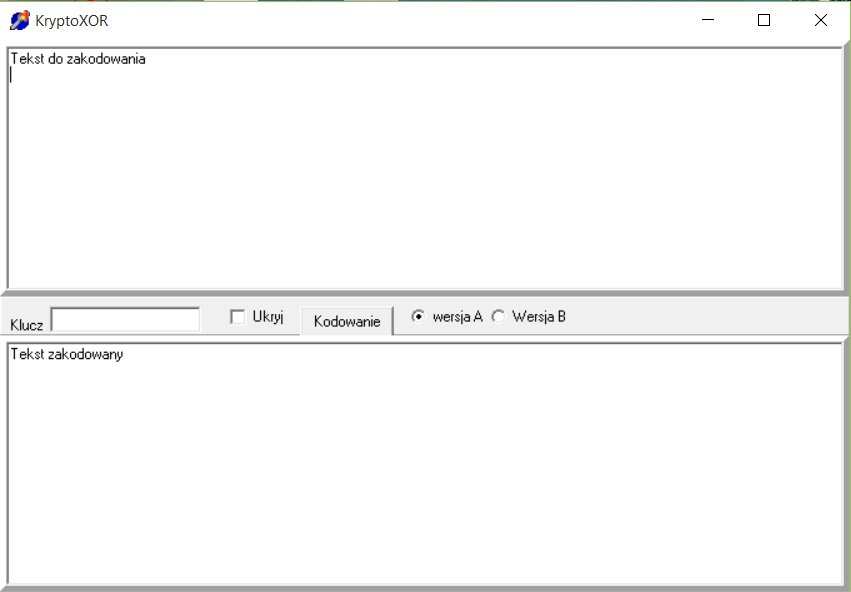
\includegraphics[scale=0.70]{Interfejs.jpg}
\caption{Interfejs programu.}%
\label{rys:etykieta}
\end{figure} 

\chapter{Wstęp teoretyczny}
Szyfr XOR to odmiana szyfru Vigenère'a. Różni się tym, że zamiast manipulować na literach i znakach, zmienia bity i bajty wiadomości przechowywanej w pamięci.

Zamiast dodawać do siebie dwie litery, jak w oryginalnej wersji, w szyfrze XOR algorytm sumuje kolejne bajty tekstu jawnego i klucza o dowolnej długości za pomocą działania XOR. Po wykorzystaniu ostatniego bajtu, przechodzi się z powrotem do pierwszego (jak w klasycznej wersji).

W celu odszyfrowania postępowanie jest takie samo, czyli dodaje się bajty klucza do bajtów szyfrogramu za pomocą operacji XOR.

Szyfrowanie i deszyfrowanie można w przedstawić za pomocą następujących wzorów:
    M XOR K = C,
    C XOR K = M

\chapter{Przebieg}
Na laboratorium mieliśmy kodować i rozkodowywać przykłądowe teksty przy wykorzystaniu wspomnianego wcześniej programu. Procedura kodowania wygląda następująco.

\begin{figure}[H]
\centering
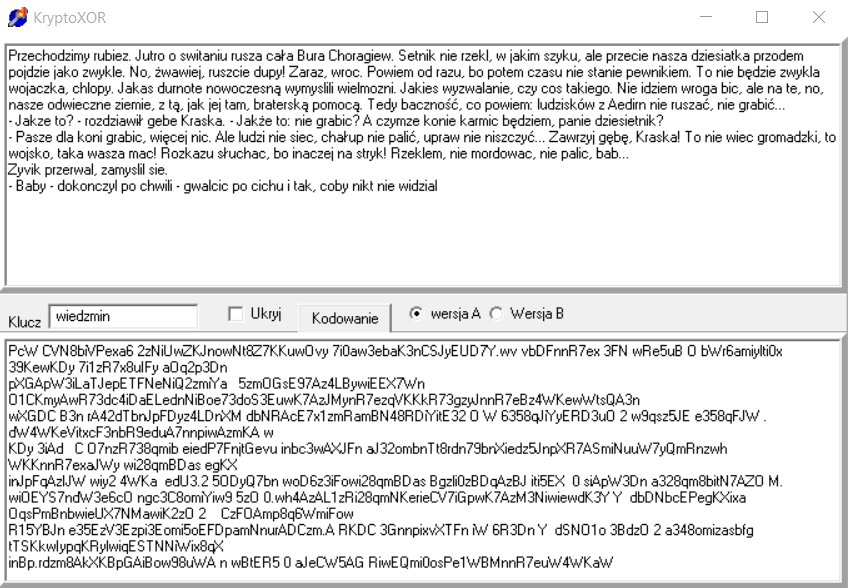
\includegraphics[scale=0.70]{kodowanie.jpg}
\caption{Kodowanie tekstu.}%
\label{rys:etykieta}
\end{figure} 

Z kolei rozkodowanie wykonuje się odwrotnie. Trzeba tylko wyliczyć lub wpaść na klucz kodujący. Litery klucza których nie znamy można zastąpić znakami zapytania.

\begin{figure}[H]
\centering
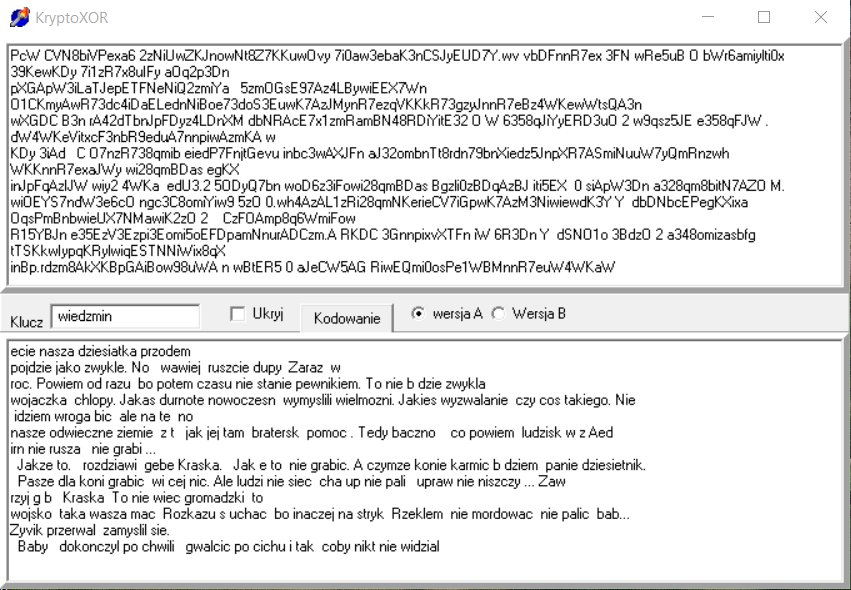
\includegraphics[scale=0.70]{rozkodowanie.jpg}
\caption{Rozszyfrowanie tekstu.}%
\label{rys:etykieta}
\end{figure} 

\chapter{Wnioski}
Szyfrowanie metodą XOR nie jest zbyt bezpieczne przy krótkich hasłach ponieważ dla komputera znalezienie szyfru jest kwestją czasu. Za to jeśli klucz jest przynajmniej tak długi jak tekst i jednorazowy powinno stanowić dużo większe wyzwanie. Jednak powstają przy okazji inne problemy związane z zarządzaniem dożą ilością kluczy i ryzykiem z tym związanym.

\end{document}
